\subsection{Learning the classifier.}\label{sec:classifier}

We have so far assumed that $g$ can combine an arbitrary subset of features and provide a distribution $P(Y = y)$---for example, a Gaussian Naive Bayes (NB) model trained on the fully-observed data.
However, a Naive Bayes classifier suffers from its restrictive independence assumptions.

Since discriminative classifiers commonly provide better performance, we use a \textbf{logistic regression} classifier, which presents a new challenge: at test time, some feature values are missing and need to be imputed.

If the classifier is trained exclusively on fully-observed data, then the feature value statistics at test time will not match, resulting in poor performance.
Therefore, we need to learn classifier weights on a distribution of data that exhibits the pattern of missing features induces by the policy $\pi$.
At the same time, learning the policy depends on the classifier $g$, used in the computation of the rewards.

\begin{algorithm}[]
\SetKwFunction{ComputeRewards}{ComputeRewards}
\SetKwFunction{GatherSamples}{GatherSamples}
\SetKwFunction{UpdatePolicy}{UpdatePolicy}
\SetKwFunction{UpdateClassifier}{UpdateClassifier}

\SetAlgoLined
\KwIn{$\mathcal{D} = \{x_n, y_n\}_{n=1}^N$; $\mathcal{L}_\mathcal{B}$}
\KwResult{Trained $\pi$, $g$}
\BlankLine
$\pi_0 \leftarrow$ random\;
\For {$i \leftarrow 1$ \KwTo max\_iterations} {
    States, Actions, Costs, Labels $\leftarrow$ \GatherSamples{$\mathcal{D}$, $\pi_{i-1}$}\;
    $g_i \leftarrow$ \UpdateClassifier{States, Labels}\;
    Rewards $\leftarrow$ \ComputeRewards{States, Costs, Labels, $g_i, \mathcal{L}_\mathcal{B}, \gamma$}\;
    $\pi_i \leftarrow$ \UpdatePolicy{States, Actions, Rewards}\;
}
\caption{Because reward computation depends on the classifier, and the distribution of states depends on the policy, $g$ and $\pi$ are trained iteratively.\label{alg:learning}}
\end{algorithm}


For this reason, the policy and classifier need to be learned jointly: \autoref{alg:learning} gives the iterative procedure.
In summary, we start from random $\pi$ and $g$, gather a batch of trajectories.
The batch is used to update both $g$ and $\pi$.
Then new trajectories are generated with the updated $\pi$, rewards are computed using the updated $g$, and the process is repeated.
This is a variant of generalized policy iteration \cite{Sutton1998}.

\paragraph{Unobserved value imputation.}
Unlike the Naive Bayes classifier, the logistic regression classifier is not able to use an arbitrary subset of features $\mathcal{H}_\pi$, but instead operates on feature vectors of a fixed size.
To represent the feature vector of a fully observed instance, we write $\mathbf{x} = [h_1(x), \dots, h_f(x)]$.
In case that $\mathcal{H}_\pi \subset \mathcal{H}$, we need to fill in unobserved feature values in the vector.

A basic strategy is \textbf{mean imputation}: filling in with the mean value of the feature:
\begin{align}
\mathbf{x}_\pi = \left[ h_i(x) : \left\{ \begin{array}{rl}
 h_i(x) &\mbox{ if $h_i \in \mathcal{H}_{\pi(x)}$} \\
 \bar{\mathbf{h}}_i &\mbox{ otherwise}
\end{array} \right. \right]
\end{align}

If we assume that $\mathbf{x}$ is distributed according to a multivariate Gaussian $\mathbf{x} \sim \mathcal{N}(\mathbf{0}, \Sigma)$, where $\Sigma$ is the sample covariance $X^T X$ and the data is standardized to have zero mean, then it is possible to do \textbf{Gaussian imputation}.
Given a feature subset $\mathcal{H}_\pi$, we write:
\begin{equation}
\mathbf{x}_\pi = \begin{bmatrix} \mathbf{x}^\text{o}\\  \mathbf{x}^\text{u} \end{bmatrix} \sim \mathcal{N} \left( \mathbf{0}, \begin{bmatrix} \mathbf{A} & \mathbf{C}\\ \mathbf{C}^T & \mathbf{B} \end{bmatrix} \right)
\end{equation}
where $\mathbf{x}^\text{o}$ and $\mathbf{x}^\text{u}$ represent the respectively observed and unobserved parts of the full feature vector $\mathbf{x}$.
%, $\mathbf{A}$ is the covariance matrix of $\mathbf{x}^\text{o}$, $\mathbf{B}$ is the covariance matrix of $\mathbf{x}^\text{u}$, and $C$ is the cross-variance matrix that has as many rows as the size of $\mathbf{x}^\text{o}$ and as many columns as the size of $\mathbf{x}^\text{u}$.
%\parencite{Roweis-gaussian-identities}.
In this case, the distribution over unobserved variables conditioned on the observed variables is given as
$\mathbf{x}^\text{u} \mid \mathbf{x}^\text{o} \sim \mathcal{N} \left( \mathbf{C}^T \mathbf{A}^{-1} \mathbf{x}^\text{o},\, \mathbf{B} - \mathbf{C}^T \mathbf{A}^{-1} \mathbf{C} \right)$.

\paragraph{Learning more than one classifier.}
As illustrated in \hyperref[fig:state_space]{Figure~\ref*{fig:state_space}}, the policy $\pi$ selects some feature subsets more frequently than others.
Instead of learning only one classifier $g$ that must be robust to all observed feature subsets, we can learn several classifiers, one for each of the most frequent subsets.
This is done by maintaining a distribution over encountered feature subsets during training.
For each of the $K$ most frequent subsets, a separate classifier is trained, using data that is closest by Hamming distance on the selected-feature bit vector.

Each classifier is trained with the \textsc{Liblinear} implementation of logistic regression, with $L_2$ regularization parameter K-fold cross-validated at each iteration.

\begin{figure}[ht]
\centering
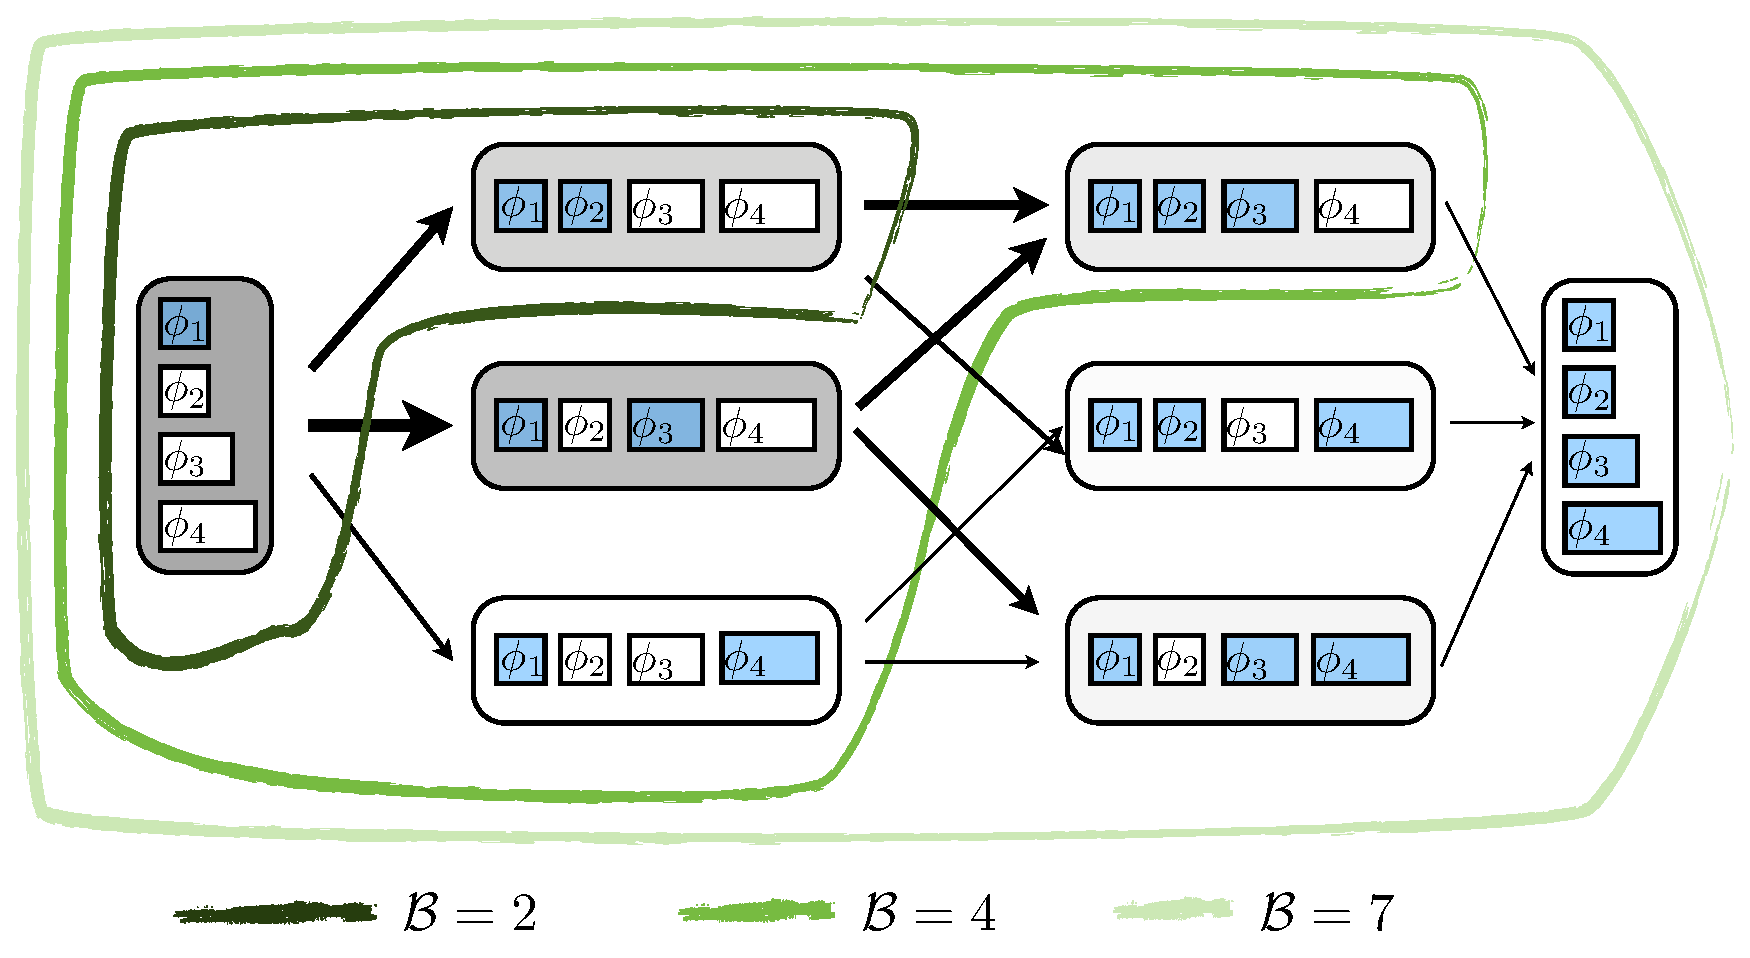
\includegraphics[width=1\linewidth]{../../figures/mdp_masks.pdf}
\caption{
The action space $\mathcal{A}$ of the MDP is the the set of features $\mathcal{H}$, represented by the $\phi$ boxes.
The primary discretization of the state space can be visualized by the possible feature subsets (larger boxes); selected features are colored in the diagram.
The feature selection policy $\pi$ induces a distribution over feature subsets, for a dataset, which is represented by the shading of the larger boxes.
Not all states are reachable for a given budget $\mathcal{B}$.
In the figure, we show three ``budget cuts'' of the state space.
\label{fig:state_space}
}
\end{figure}
